%%%%%%%%%%%%%%%%%%%%%%%%%%%%%%%%%%%%%%%%%%%%%%%%%%%%%%%%%%%%%%%%%%%%%%%%
%% Customizações do abnTeX2 (http://abnTeX2.googlecode.com)           %%
%% para a Universidade Federal do Ceara - UFC                         %%
%% baseado no ueceTex2                                                %%
%% This work may be distributed and/or modified under the             %%
%% conditions of the LaTeX Project Public License, either version 1.3 %%
%% of this license or (at your option) any later version.             %%
%% The latest version of this license is in                           %%
%%   http://www.latex-project.org/lppl.txt                            %%
%% and version 1.3 or later is part of all distributions of LaTeX     %%
%% version 2005/12/01 or later.                                       %%
%%                                                                    %%
%% This work has the LPPL maintenance status `maintained'.            %%
%%                                                                    %%
%% The Current Maintainer of this work is:                            %%
%%  Alexsandro Oliveira Alexandrino                                   %%
%%                                                                    %%
%% Project available on:                                              %%
%% https://github.com/sandrooliveira1501/template-tcc2                %%
%%                                                                    %%
%% Further information about abnTeX2                                  %%
%% are available on http://abntex2.googlecode.com/                    %%
%%                                                                    %%
%%%%%%%%%%%%%%%%%%%%%%%%%%%%%%%%%%%%%%%%%%%%%%%%%%%%%%%%%%%%%%%%%%%%%%%%

\documentclass[
    a4paper,          % Tamanho da folha A4
    %sumario=tradicional, %outra opção de sumário
    12pt,             % Tamanho da fonte 12pt
    chapter=TITLE,    % Todos os capitulos devem ter caixa alta
    section=title,    % Todas as secoes devem ter caixa normal
    oneside,          % Usada para impressao em apenas uma face do papel
    english,          % Hifenizacoes em ingles
    spanish,          % Hifenizacoes em espanhol
    brazil            % Ultimo idioma eh o idioma padrao do documento
]{abntex2}

%%%%%%%%%%%%%%%%%%%%%%%%%%%%%%%%%%%%%%%%%%%%%%%%%%%%%%%%%%%%%%%%%%%%%%%%
%% Customizações do abnTeX2 (http://abnTeX2.googlecode.com)           %%
%% para a Universidade Federal do Ceara - UFC                         %%
%% baseado no ueceTex2                                                %%
%% This work may be distributed and/or modified under the             %%
%% conditions of the LaTeX Project Public License, either version 1.3 %%
%% of this license or (at your option) any later version.             %%
%% The latest version of this license is in                           %%
%%   http://www.latex-project.org/lppl.txt                            %%
%% and version 1.3 or later is part of all distributions of LaTeX     %%
%% version 2005/12/01 or later.                                       %%
%%                                                                    %%
%% This work has the LPPL maintenance status `maintained'.            %%
%%                                                                    %%
%% The Current Maintainer of this work is:                            %%
%%  Alexsandro Oliveira Alexandrino                                   %%
%%                                                                    %%
%% Project available on:                                              %%
%% https://github.com/sandrooliveira1501/template-tcc2                %%
%%                                                                    %%
%% Further information about abnTeX2                                  %%
%% are available on http://abntex2.googlecode.com/                    %%
%%                                                                    %%
%%%%%%%%%%%%%%%%%%%%%%%%%%%%%%%%%%%%%%%%%%%%%%%%%%%%%%%%%%%%%%%%%%%%%%%%

% \documentclass[
%     a4paper,          % Tamanho da folha A4
%     12pt,             % Tamanho da fonte 12pt
%     chapter=TITLE,    % Todos os capitulos devem ter caixa alta
%     section=TITLE,    % Todas as secoes devem ter caixa alta
%     oneside,          % Usada para impressao em apenas uma face do papel
%     english,          % Hifenizacoes em ingles
%     spanish,          % Hifenizacoes em espanhol
%     brazil            % Ultimo idioma eh o idioma padrao do documento
% ]{abntex2}

% Importações de pacotes
\usepackage[utf8]{inputenc}                         % Acentuação direta
\usepackage[T1]{fontenc}                            % Codificação da fonte em 8 bits
\usepackage{graphicx}                               % Inserir figuras
\usepackage{amsfonts, amssymb, amsmath}             % Fonte e símbolos matemáticos
\usepackage{booktabs}                               % Comandos para tabelas
\usepackage{verbatim}                               % Texto é interpretado como escrito no documento
\usepackage{multirow, array}                        % Múltiplas linhas e colunas em tabelas
\usepackage{indentfirst}                            % Endenta o primeiro parágrafo de cada seção.
\usepackage{listings}                               % Utilizar codigo fonte no documento
\usepackage{xcolor}
\usepackage{microtype}                              % Para melhorias de justificação?
\usepackage[portuguese,ruled,lined]{algorithm2e}    % Escrever algoritmos
\usepackage{algorithmic}                            % Criar Algoritmos
\usepackage{amsgen}
\usepackage{lipsum}                                 % Usar a simulação de texto Lorem Ipsum
%\usepackage{titlesec}                               % Permite alterar os títulos do documento
\usepackage{tocloft}                                % Permite alterar a formatação do Sumário
\usepackage{etoolbox}                               % Usado para alterar a fonte da Section no Sumário
\usepackage[nogroupskip,nonumberlist,acronym]{glossaries}                % Permite fazer o glossario
\usepackage{caption}                                % Altera o comportamento da tag caption
%\usepackage[alf, abnt-emphasize=bf, bibjustif, recuo=0cm, abnt-etal-cite=2, abnt-etal-list=0]{abntex2cite}  % Citações padrão ABNT
\usepackage[alf, abnt-emphasize=bf, bibjustif, recuo=0cm, abnt-etal-cite=3, abnt-etal-list=0]{abntex2cite} %Citação ABNT-UFC
%\usepackage[bottom]{footmisc}                      % Mantém as notas de rodapé sempre na mesma posição
%\usepackage{times}                                 % Usa a fonte Times
\usepackage{mathptmx}                               % Usa a fonte Times New Roman
%\usepackage{lmodern}                               % Usa a fonte Latin Modern
%\usepackage{subfig}                                % Posicionamento de figuras
%\usepackage{scalefnt}                              % Permite redimensionar tamanho da fonte
%\usepackage{color, colortbl}                       % Comandos de cores
%\usepackage{lscape}                                % Permite páginas em modo "paisagem"
%\usepackage{ae, aecompl}                           % Fontes de alta qualidade
%\usepackage{picinpar}                              % Dispor imagens em parágrafos
%\usepackage{latexsym}                              % Símbolos matemáticos
%\usepackage{upgreek}                               % Fonte letras gregas
\usepackage{appendix}                               % Gerar o apendice no final do documento
\usepackage{paracol}                                % Criar paragrafos sem identacao
\usepackage{lib/ufctex2}		                    % Biblioteca com as normas da UFC para trabalhos academicos
\usepackage{pdfpages}                               % Incluir pdf no documento
\usepackage{amsmath}                                % Usar equacoes matematicas
\usepackage{titlesec}                               % modificação de títulos

% Organiza e gera a lista de abreviaturas, simbolos e glossario
\makeglossaries

% Gera o Indice do documento
\makeindex

\usepackage{float}

%%%%%%%%%%%%%%%%%%%%%%%%%%%%%%%%%%%%%%%%%%%%%%%%%%%%%
%%          Configuracoes do ufcTex2               %%
%%%%%%%%%%%%%%%%%%%%%%%%%%%%%%%%%%%%%%%%%%%%%%%%%%%%%

% Opcoes disponiveis

\trabalhoacademico{tccgraduacao}

% Define se o trabalho eh uma qualificacao
% Coloque 'nao' para versao final do trabalho

\ehqualificacao{nao}

% Remove as bordas vermelhas e verdes do PDF gerado
% Coloque 'sim' pare remover

\removerbordasdohyperlink{sim}

% Adiciona a cor Azul a todos os hyperlinks

\cordohyperlink{nao}

%%%%%%%%%%%%%%%%%%%%%%%%%%%%%%%%%%%%%%%%%%%%%%%%%%%%%
%%          Informação sobre a IES                 %%
%%%%%%%%%%%%%%%%%%%%%%%%%%%%%%%%%%%%%%%%%%%%%%%%%%%%%

\ies{Universidade Federal do Ceará}
\iessigla{UFC}
\centro{Campus Quixadá}

%%%%%%%%%%%%%%%%%%%%%%%%%%%%%%%%%%%%%%%%%%%%%%%%%%%%%
%%        Informação para TCC de Graduacao         %%
%%%%%%%%%%%%%%%%%%%%%%%%%%%%%%%%%%%%%%%%%%%%%%%%%%%%%

%Substituir pelo seu curso
\graduacaoem{Ciência da Computação}
\habilitacao{bacharel}
\tipohabilitacao{Bacharelado}

%%%%%%%%%%%%%%%%%%%%%%%%%%%%%%%%%%%%%%%%%%%%%%
%%  Informação relacionadas ao trabalho     %%
%%%%%%%%%%%%%%%%%%%%%%%%%%%%%%%%%%%%%%%%%%%%%%

\autor{Jhonata Adam Silva Matias}
\titulo{Título do Trabalho: Subtítulo}
\data{2016}
\local{Quixadá -- Ceará}

% Exemplo: \dataaprovacao{01 de Dezembro de 2016}
\dataaprovacao{}

%%%%%%%%%%%%%%%%%%%%%%%%%%%%%%%%%%%%%%%%%%%%%
%%     Informação sobre o Orientador       %%
%%%%%%%%%%%%%%%%%%%%%%%%%%%%%%%%%%%%%%%%%%%%%

\orientador{Nome do seu Orientador}
\orientadories{Universidade Federal do Ceará – UFC}
\orientadorcentro{Campus Quixadá}
\orientadorfeminino{nao} % Coloque 'sim' se for do sexo feminino

%%%%%%%%%%%%%%%%%%%%%%%%%%%%%%%%%%%%%%%%%%%%%
%%      Informação sobre o Co-orientador   %%
%%%%%%%%%%%%%%%%%%%%%%%%%%%%%%%%%%%%%%%%%%%%%

% Deixe o nome do coorientador em branco para remover do documento

\coorientador{Nome Co-orientador}
\coorientadories{Universidade Federal do Ceará - UFC}
\coorientadorcentro{Campus Quixadá}
\coorientadorfeminino{nao} % Coloque 'sim' se for do sexo feminino

%%%%%%%%%%%%%%%%%%%%%%%%%%%%%%%%%%%%%%%%%%%%%
%%      Informação sobre a banca           %%
%%%%%%%%%%%%%%%%%%%%%%%%%%%%%%%%%%%%%%%%%%%%%

% Atenção! Deixe o nome do membro da banca para remover da folha de aprovacao

% Exemplo de uso:
% \membrodabancadois{Prof. Dr. Fulano de Tal}
% \membrodabancadoisies{Universidade Federal do Ceará - UFC}

\membrodabancadois{Membro da Banca Dois}
\membrodabancadoiscentro{Campus Quixadá}
\membrodabancadoisies{Universidade Federal do Ceará - UFC}
\membrodabancatres{Membro da Banca Três}
\membrodabancatrescentro{Campus Quixadá}
\membrodabancatresies{Universidade Federal do Ceará - UFC}
%\membrodabancaquatro{Membro da Banca Quatro}
%\membrodabancaquatrocentro{Centro de Ciências e Tecnologia - CCT}
%\membrodabancaquatroies{Universidade Federal do Ceará - UFC}
%\membrodabancacinco{Membro da Banca Cinco}
%\membrodabancacincocentro{Teste}
%\membrodabancacincoies{Universidade do Membro da Banca Cinco - SIGLA}
%\membrodabancaseis{Membro da Banca Seis}
%\membrodabancaseiscentro{}
%\membrodabancaseisies{Universidade do Membro da Banca Seis - SIGLA}

%%COMENTE TUDO QUE NÃO FOR UTILIZAR

\begin{document}
    
    % referencia com parênteses as equações
	\let\oldref\ref
	\renewcommand{\ref}[1]{(\oldref{#1})}   
    
    \captionsetup[figure]{slc=off}

    %% CORREÇÃO DE TÍTULOS
    \titleformat{\section}
    {\normalfont\normalsize\bfseries}{\thesection}{1em}{}
    \titleformat{\subsection}
    {\normalfont\normalsize\bfseries\itshape}{\thesubsection}{1em}{}
    \titleformat{\subsubsection}
    {\normalfont\normalsize\itshape}{\thesubsubsection}{1em}{}
    \titleformat{\subsubsubsection}
    {\normalfont\normalsize\itshape}{\thesubsubsubsection}{1em}{}
    %%ADICIONE MAIS CASO NECESSÁRIO


	% Elementos pré-textuais
	\imprimircapa
	\imprimirfolhaderosto{}
	%Substitua o pdf da ficha pelo seu próprio
	\imprimirfichacatalografica{elementos-pre-textuais/ficha-catalografica}
	%\imprimirerrata{elementos-pre-textuais/errata}
	\imprimirfolhadeaprovacao
	\imprimirdedicatoria{elementos-pre-textuais/dedicatoria}
	\imprimiragradecimentos{elementos-pre-textuais/agradecimentos}
	\imprimirepigrafe{elementos-pre-textuais/epigrafe}
	\imprimirresumo{elementos-pre-textuais/resumo}
	\imprimirabstract{elementos-pre-textuais/abstract}
	%Insira apenas os utilizados
	\imprimirlistadeilustracoes
	\imprimirlistadetabelas
	\imprimirlistadequadros
	%\imprimirlistadealgoritmos
	%\imprimirlistadecodigosfonte
	%\imprimirlistadeabreviaturasesiglas % funciona apenas usando o makefile
	\imprimirlistadeabreviaturasesiglasaux{elementos-pre-textuais/lista-de-abreviaturas-siglas-aux} % opcional
	\imprimirlistadesimbolos{elementos-pre-textuais/lista-de-simbolos} % opcional
	\imprimirsumario

	%Elementos textuais
	\textual
	%Sugestão de capítulos e ordem entre eles, sinta-se a vontade para alterar
	%%
%%  O texto deste template é de autoria da professora Tania Saraiva de Melo Pinheiro (Universidade Federal do Ceará - Campus Quixadá)
%%
%%
%%
%%
%%

\chapter{Introdução}

Antes do início de um semestre letivo, as universidades realizam uma série de tarefas afim de se preparar para as atividades de um novo semestre. Entre essas tarefas se encontra a alocação de professores em disciplinas, que lida com o problema de alocar professores em disciplinas e disciplinas nos horários de aula respeitando um conjunto de restrições. O problema se torna difícil de resolver quando lidamos com um grande volume de dados. Isso se dá por alguns motivos, que vão desde a quantidade de restrições envolvidas até as preferências concorrentes dos professores. Doravante, chamaremos esse problema de \textbf{PAPD (problema de alocação de professores em disciplinas)}.

No campus da \textbf{Universidade Federal do Ceará em Quixadá (UFC-Quixadá)}, a direção do campus e os coordenadores de curso participam da definição da grade de horários acadêmicos. Nela está definida toda a alocação do campus, tanto de professores em disciplinas quanto de disciplinas na grade de horários. Atualmente as ofertas de disciplinas são definidas por cada curso. São definidos de forma manual a alocação dos professores à cada oferta, e de forma automatizada a alocação das disciplinas nos horários de aula. Essa alocação é feita respeitando um conjunto de restrições que definem como os professores e as disciplinas devem ser alocados.

Dentro do contexto de uma Universidade, conseguimos identificar três grupos de pessoas que são diretamente afetadas pelo PAPD, seja pela alocação gerada ou pelo método utilizado para fazer a alocação. São eles: os professores, os alunos e os responsáveis por gerar a alocação. Os professores têm suas preferências quanto às disciplinas que vão ministrar. Os alunos por sua vez, são diretamente afetados por uma alocação que coloque em choque os horários de duas ou mais disciplinas que eles desejam cursar. Quanto aos responsáveis pela alocação, esses lidam com um volume de trabalho que cresce de forma exponencial em função da quantidade de dados envolvidos na alocação. Automatizar a resolução do PAPD, maximizando a preferência geral dos professores e as opções de matrícula dos alunos é vantajoso para todas as pessoas afetadas pelo problema.

Uma larga variedade de problemas de alocação voltados a escolas de ensino médio e universidades são encontrados na literatura, bem como diversas abordagens são propostas para resolver o problema, dentre elas: Algorítimos Genéticos, Satisfação de Restrições, Fluxo em Redes e Programação Inteira, entre outras \cite{schaerf1999survey}. Neste trabalho, modelamos o PAPD como um problema de Programação Inteira. 

Um problema de Programação Inteira consiste em um conjunto de variáveis que compõem uma função objetivo e um conjunto de equações ou inequações lineares que são as restrições do problema. Resolver um problema de Programação Inteira, se resume a encontrar uma valor inteiro para as variáveis, que satisfaça todas as restrições e minimizes\footnote{Ou maximize, dependendo da natureza do problema.} o custo da função objetivo.

Este trabalho teve como objetivo geral produzir um modelo de Programação Inteira capaz de resolver o PAPD aplicado à UFC-Quixadá. Para tanto, identificamos as restrições que são utilizadas no processo de alocação. A partir das restrições levantadas, modelamos o PAPD como um problema de Programação Inteira e realizamos alguns teste implementando o modelo e verificando o tempo que ele leva para resolver o problema para instâncias de diferentes tamanhos.

No trabalho de \citeonline{naadriano}, é proposta uma forma de modelar o PAPD a partir dos conceitos da Teoria dos Jogos. Esse trabalho também leva em conta as restrições da alocação da UFC-Quixadá de forma que uma solução do modelo proposto no trabalho, satisfaz essas restrições considerando a preferência por disciplinas dos professores. Assim como no trabalho de \citeonline{naadriano}, nosso trabalho leva em conta as restrições da alocação da UFC-Quixadá para produzir um modelo e maximiza a preferência por disciplinas dos professores. A diferença entre os dois trabalhos se encontra na abordagem utilizada para resolver o problema e na maximização das opções de matrícula que realizamo no nosso trabalho. 

\citeonline{lach2012curriculum} apresentam um modelo de Programação Inteira baseado no conjunto de restrições das instâncias da \textit{2nd International Timetabling Competition} \cite{itc}. Esse modelo resolve as instâncias em dois passos: primeiro  associa disciplinas com seus horários e depois associa esses horários as salas de aula. O que é importante ressaltar da abordagem é que ela trata o problema com dois tipos de restrições: \textit{Hard} e \textit{Soft}. Restrições \textit{Hard} devem ser respeitadas incondicionalmente, por outro lado, restrições \textit{Soft} devem ser satisfeitas tanto quanto possível. \citeonline{lach2012curriculum}, assim como no nosso trabalho, trabalham com Programação Inteira para resolver o problema de alocação em universidades. Os dois trabalhos se diferem na forma como resolvem problema, pois o nosso trabalho não divide em passos o processo de resolução. Além disso, os dois trabalhos lidam com um conjunto de restrições diferentes.

Esse trabalho está dividido em cinco capítulos. No Capítulo 2, é apresentada a fundamentação teórica. O Capítulo 3 apresenta o modelo de Programação Inteira desenvolvido para o PAPD. O Capítulo 4 apresenta a avalização feita sobre o modelo desenvolvido. E por fim, no Capítulo 5, são feitas as considerações finais e as indicações de trabalhos futuros.

	
	%\chapter{Trabalhos Relacionados}

No cotidiano, um bom ponto de partida para se resolver um problema é procurar soluções já existentes para utilizá-las. Costumeiramente, as soluções que já existentes não se aplicam diretamente ao nosso caso, precisando ser adaptadas. Assim, antes de se começar a resolver questões de pesquisa, é preciso conhecer o que existe de mais atual no seu tema. 

Usando a abordagem de \citeonline{wazlawick2014metodologia} para explicar a necessidade de se conhecer a área de estudo, cabe lembrar que antes de se construir uma nova ponte é importante conhecer os tipos de pontes que já existem; é preciso conhecer qual a atualidade do assunto estudado. Do contrário, pode estar construindo uma catapulta achando que se trata da melhor forma de atravessar um rio!

Para conhecer a atualidade do tema de estudo proposto, o ideal seria fazer o vasto levantamento do que se tem estudado ou praticado sobre o tema. Entretanto, em cursos de graduação em geral não há tempo para tanto, a menos que o objeto do estudo seja justamente o levantamento do estado da arte. 
Na impossibilidade de realiza-lo, deve-se pelo menos fazer um levantamento por amostragem. Tal amostra consiste de um conjunto de trabalhos relacionados: uma boa seleção de textos encontrados em periódicos e eventos relevantes para a área estudada.  O levantamento é facilitado quando se encontram materiais denominados surveys (levantamentos), podendo ser compilações de:

\begin{alineascomponto}
    \item \textbf{Estado-da-arte}: artigos que apresentem conceitos mais recentes, estabelecidos na literatura científica;
    \item \textbf{Estado-da-prática}: semelhante ao anterior, mas com foco no que está estabelecido atualmente como status quo da prática profissional.
\end{alineascomponto}

Na escrita desta seção, deve-se evitar usar a palavra “trabalho” para se referir tanto à própria pesquisa quanto à de outro autor, sugere-se:

\begin{alineascomponto}
\item em vez de “o trabalho de Bittar (2001) prevê que ...”,
\item utilizar-se simplesmente “Bittar (20010 prevê que....”.
\end{alineascomponto}

Apenas a partir do momento em que se conhece o estado da arte (ou prática), seja plenamente ou por uma amostra de trabalhos relacionados, é que o pesquisador está pronto para adequadamente identificar e possíveis pesquisas a serem realizadas. O anúncio de seus objetivos, portanto, ocorre após tecer considerações sobre o estado do conhecimento ou prática em sua área de estudo.

\section{Quando parece ser cabível o inverso}

Em algumas situações, o pesquisador tende a apresentar primeiro seu objeto de estudo e apenas depois o estado da arte. Observa-se que tais situações ocorrem quando o problema de pesquisa é extraído do cotidiano do pesquisador. Por exemplo: “não estou conseguindo bom resultado com determinado processo de trabalho, e vou pesquisar como melhorá-lo”.

Nesta situação, há uma tendência a primeiro se definir objetivo e só depois fazer um levantamento do estado da arte/prática. Mas qual seria então o propósito do tal levantamento? Buscar soluções semelhantes que auxiliem na elaboração da solução buscada? Se assim o for, então tais trabalhos relacionados não estariam também contribuindo para um refinamento na definição dos objetivos da pesquisa?
	\chapter{Fundamentação Teórica}
\label{cap:fundamentacao-teorica}

Esta Seção contém os conceitos que fundamentarão as análises. Por exemplo, se será feita a avaliação de algum artefato, aqui se deve caracterizar quais aspectos deste artefato serão considerado, ou seja, quais os critérios de análise a serem considerados no trabalho. Também se informa qual o valor desejável para cada um desses critérios.

A fundamentação teórica NÃO é um glossário de termos, em que o autor comprova que os compreende. Sua função é deixar claro qual o significado adotado para cada conceito utilizado em sua pesquisa. Por exemplo, o que é Computação em Nuvem no seu trabalho? Você abordará questões de software ou de infraestrutura, ou a visão do usuário final? Caso existam diferentes abordagens para um mesmo conceito, deixe claro qual aquela que será adotada. 

O título desta Seção pode ser alterado de “Fundamentação Teórica” para algum tema central do seu trabalho. Tipicamente, ela contém muitas citações indicando os autores que guiaram sua elaboração. Na sequência, há muitos exemplos de como se referir e citar os textos utilizados.


\section{Título de seção }


Texto texto texto texto texto texto texto texto texto texto texto texto texto texto texto texto texto texto texto texto texto texto texto texto texto texto texto texto texto texto texto texto texto texto texto texto texto texto texto texto texto texto texto texto texto.

\subsection{Título da seção terciária}

Texto texto texto texto texto texto texto texto texto texto texto texto texto texto texto texto texto texto texto texto texto texto texto texto texto texto texto texto texto texto texto texto texto texto texto texto texto texto texto texto texto texto texto texto texto.

\subsubsection{Título da seção quaternária}

Texto texto texto texto texto texto texto texto texto texto texto texto texto texto texto texto texto texto texto texto texto texto texto texto texto texto texto texto texto texto texto texto texto texto texto texto texto texto texto texto texto texto texto texto texto.
	\chapter{Modelo para o PAPD da UFC-Quixadá}
\label{cap:modelo-para-o-papd}

A construção de um modelo de PI para o problema de alocação de professores da UFC-Quixadá demanda o conhecimento de algumas informações relevantes no domínio do problema. Dessa forma, foi feito um levantamento de como é realizada atualmente a alocação na UFC-Quixadá, e chegamos às informações que são importantes para a alocação dos professores e das disciplinas. 

A alocação é feita sobre uma grade de horários semanal. Cada elemento dessa grade representa um horário disponível para alocação ao qual chamamos de \textbf{\textit{slot}}. Um \textit{slot} tem o valor de dois créditos (2 horas), ou seja, uma disciplinas de quatro créditos demanda dois \textit{slots} para ser alocada. Um único dia agrupa seis \textit{slots}, os quais estão divididos nos três turnos de um dia (manhã, tarde e noite). Um turno de um dia agrupa dois \textit{slots}, o \textit{slot} AB e o \textit{slot} CD do turno. 

Neste trabalho, mapeamos os \textit{slots} para valores inteiros, dessa forma os \textit{slots} da segunda-feira são representados pelos valores: 1, 2, 3, 4, 5 e 6; os da terça-feira: 7, 8, 9, 10, 11 e 12; e assim por diante. A tabela abaixo mostra de forma completa como os \textit{slots} estão organizados na grade de horários.

\begin{figure}[htbp]
	\centering
	\IBGEtab{
		\Caption{\label{figura-1}Grade de horários e seus respectivos \textit{slots}.}		
    }{
		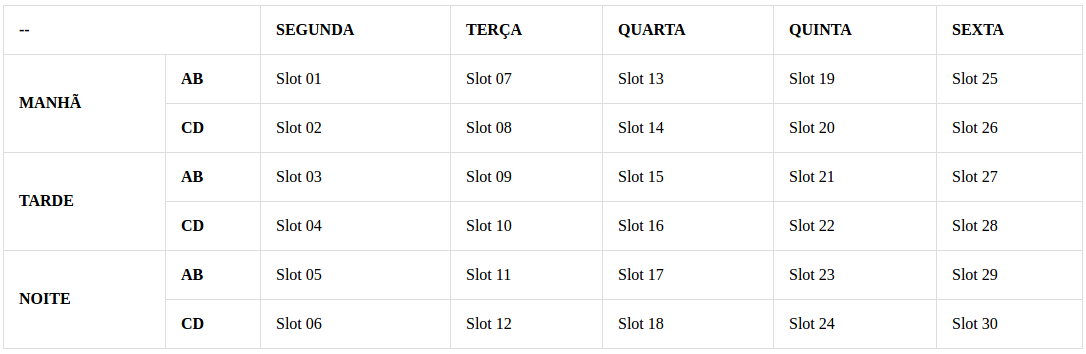
\includegraphics[scale=0.40]{figuras/tabela-de-slots}
	}{
	\Fonte{Elaborada pelo autor}
}
\end{figure}


Para os professores, há uma carga horária máxima e mínima para cumprir. Essa carga horária pode ser diferente para cada professor, já que alguns professores realizam atividades como coordenação de curso, que permitem redução de carga horária. O número de disciplinas que um professor deve ser associado depende então de sua carga horário máxima e mínima e do número de créditos das disciplinas. 

Há também restrições que definem os horários e os dias aos quais os professores não devem ser alocados:

\begin{alineascomponto}
\item professores não devem ser alocados nos três turnos de um mesmo dia (essa restrição pode ser quebrada desde que autorizado por escrito pelo professor. Mantivemos obrigatória para todos os professores em nossa implementação);
\item professores não devem ser alocados no último horário de um dia e no primeiro horário do dia seguinte;
\item professores devem estar livres no horário CD da manhã ou no AB da tarde de quarta (para os encontros denominados ``seminários'');
\item um professor deve ter a segunda-feira ou a sexta-feira live;
\item o dia livre (segunda-feira ou sexta-feira) é o mesmo para casais de professores;
\item professores não devem ser alocados a nenhuma disciplina nos horários das reuniões que participam.
\end{alineascomponto}

A UFC-Quixadá conta atualmente com seis cursos de graduação. Todo semestre os cursos ofertam um conjunto de disciplinas, de forma que as disciplinas a serem alocadas em um semestre são as ofertadas pelos cursos. As disciplinas estão agrupadas nesses cursos de forma que algumas delas são compartilhadas entre cursos e outras não. Embora essas disciplinas sejam compartilhadas, cada oferta é específica de um curso. 

A maioria dos cursos são de horário integral, ou seja, utilizam os turnos da manhã e da tarde para alocar suas disciplinas. Porém cada curso opta por um horário preferencial, onde a maioria das disciplinas obrigatórias são alocadas. Em alguns casos, a soma de créditos das disciplinas obrigatórias de um semestre de um cursos excede a quantidade de créditos de um turno (10 créditos). Para resolver isso os cursos optam por alocar os créditos excedentes em outro turno, já que é imprescindível que disciplinas obrigatórias de um mesmo semestre não choquem horário. Para representar isso em nosso modelo definimos um horário primário e um horário secundário para cada curso. O horário primário é onde são alocadas as disciplinas obrigatórias, e o secundário é onde são alocadas as disciplinas obrigatórias excedentes. As disciplinas optativas são livres para serem alocadas em qualquer horário.

Assim como os professores, as disciplinas têm seu conjunto de restrições:

\begin{alineascomponto}
\item uma disciplina tem um número fixo de professores que devem ser associados a ela;
\item disciplinas associadas a um mesmo professor não compartilham \textit{slots};
\item disciplinas obrigatórias de um mesmo semestre de um mesmo curso não devem compartilhar \textit{slots};
\item o número de \textit{slots} em que uma disciplina deve ser alocada é igual à metade de seus créditos;
\item uma disciplina pode ter seus horários prefixados;
\item uma disciplina deve compartilhar \textit{slots} com um conjunto prefixado de disciplinas.  
\end{alineascomponto} 

O modelo de PI proposto neste trabalho foi então construído a partir das restrições do problema. O modelo representa as entidades a serem alocadas da seguinte forma: variáveis binárias representam a associação professores/disciplinas e disciplinas/horários (ou \textit{slots}, como chamaremos neste trabalho). Por exemplo: o valor de uma variável $z_{pi}$ é 1 se o professor $p$ está associado à disciplina $i$, e 0 caso contrário. Dessa forma, estão sendo mapeados professores, disciplinas e \textit{slots} para variáveis binárias. Essas compõem as equações e inequações lineares das restrições do modelo.

Definimos que há \textbf{choque de horários} entre duas disciplinas quando elas compartilham pelo menos um \textit{slot}.

A seguir estão as variáveis, parâmetros e conjuntos presentes no modelo. Em seguida, serão apresentadas as restrições e a função objetivo.

Conjuntos:

\begin{alineascomponto}
    \item $P$ - professores;
    \item $D$ - disciplinas;
    \item $D_p$ - disciplinas do professor $p$;
    \item $C$ - cursos;
    \item $K_c$ - semestres de um curso $c$;
    \item $D_{kc}^{ob}$ - disciplinas obrigatórias de um semestre $k$ de um curso $c$;
    \item $D_{c}^{op}$ - disciplinas optativas de um curso $c$;
	\item $S$ - \textit{slots};
	\item $S_{pri_c}$ - \textit{slots} do turno primário do curso $c$;
	\item $S_{sec_c}$ - \textit{slots} do turno secundário do curso $c$;
	\item $T_i$ - disciplinas às quais a disciplina $i$ deve compartilhar \textit{slots};
	\item $H_i$ - \textit{slots} prefixados da disciplina $i$;
	\item $R$ - reuniões;
	\item $P_r$ - professores da reunião $r$;
	\item $S_r$ - \textit{slots} da reunião $r$;
	\item $A$ - casais de professores;
	\item $G_m$ - grupos de \textit{slots} de tamanho $m$.
\end{alineascomponto}

Parâmetros:

\begin{alineascomponto}
	\item $max_p$ - número máximo de créditos do professor $p$;
    \item $min_p$ - número mínimo de créditos do professor $p$;
	\item $a_{ij}$ - número de alunos que podem cursar as disciplinas $i$ e $j$;
	\item $b_{pi}$ - nível de preferência do professor $p$ pela disciplina $i$;	
	\item $crd_i$ - número de créditos da disciplina $i$;
	\item $n_i$ - número de professores na disciplina $i$;
\end{alineascomponto}

Variáveis:

\begin{alineascomponto}
    \item $x_{ij}$ - 1 se as disciplinas  $i$ e $j$ compartilham \textit{slot}, 0 caso contrário;
	\item $y_{is}$ - 1 se a disciplina $i$ está alocada no \textit{slot} $s$, 0 caso contrário
	\item $w_{ps}$ - 1 se o professor $p$ está associado ao \textit{slot} $s$, 0 caso contrário;
	\item $z_{pi}$ - 1 se o professor $p$ está associado à disciplina $i$, 0 caso contrário;
	\item $u_{kc}$ - 1 se todas as disciplinas obrigatórias do semestre $k$ do curso $c$ estão alocadas no turno primário do próprio curso;
	\item $v_p$ - 1 se o professor $p$ não dá aula na sexta-feira, 0 se não dá aula na segunda-feira.
\end{alineascomponto} 

A função objetivo define qual alocação é melhor. Para isso ela leva em conta a preferência geral dos professores e os choques de horários das disciplinas. O somatório $\sum a_{ij} * x_{ij}$ representa, na função objetivo, a soma dos alunos que podem se matricular em disciplinas que compartilham \textit{slots}. O somatório $\sum b_{pi} * z_{pi}$ representa a soma das preferências dos professores. É importante notar que a preferência de um professor por uma disciplinas só é contabilizada se ele estiver associado a essa disciplinas.

É utilizado na função objetivo um parâmetro $\alpha\in[0,1]$. Esse valor balanceia os pesos dos dois lados da função objetivo. Por exemplo, quando $\alpha = 0$, é considerado na função objetivo apenas a preferência dos professores, e ignorado o número de alunos que podem fazer pares de disciplinas que compartilham \textit{slots}. Por outro lado, se $\alpha = 1$, é considerado apenas o número de alunos nos choques de horários. Assim, para $\alpha = 0.5$, é dado peso igual para ambos.

\emph{Função Objetivo:}
$$
\min{\alpha * \sum a_{ij} * x_{ij} + (\alpha-1) * \sum b_{pi} * z_{pi}}
$$

As Restrições \ref{r1} e \ref{r2} definem, respectivamente, a carga horária máxima e mínima de cada professor.
\begin{eqnarray}
\label{r1}
\sum_{i\in{D}}^{}{crd_i * z_{pi}} \le max_p, \forall{p}\in{P} &&\\
\label{r2}
\sum_{i\in{D}}^{}{crd_i * z_{pi}} \ge min_p, \forall{p}\in{P} &&
\end{eqnarray}

A Restrição \ref{r3} impede que professores estejam alocados nos três turnos de um mesmo dia. Apresentaremos essa restrição em sua forma não linear para facilitar o entendimento do modelo, embora seja possível torná-la linear.
\begin{eqnarray}
\label{r3}
\sum_{q\in\{{0,2,4}\}}^{}{max(w_{p(s+q)}, w_{p(s+q+1)})}  \leq 2, \forall{s}\in{\{1,7,13,19,25\}}, \forall{p}\in{P}  &&
\end{eqnarray}

A Restrição \ref{r4} define que professores não devem ser alocados no último horário de um dia e no primeiro do dia seguinte.
\begin{eqnarray}
\label{r4}
w_{ps} + w_{p(s+1)}  \leq 1, \forall{s}\in{\{6, 12, 18, 24\}}, \forall{p}\in{P}  &&
\end{eqnarray}

A Restrição \ref{r5} se refere aos seminários, em que os professores devem estar livres no horário CD da manhã ou no AB da tarde de quarta.
\begin{eqnarray}
\label{r5}
w_{p14} + w_{p15} \leq 1, \forall{p\in{P}} &&
\end{eqnarray}

As Restrições \ref{r6} e \ref{r7} definem que um professor deve ter a segunda-feira ou a sexta-feira livre.
\begin{eqnarray}
\label{r6}
\sum_{s\in\{{1, 2, ..., 6}\}}{w_{ps}} \leq 6*v_p, \forall{p \in{P}} &&\\
\label{r7}
\sum_{s\in\{{25, 26, ..., 30}\}}{w_{ps}} \leq 6*(1-v_p), \forall{p \in{P}} &&
\end{eqnarray}

A Restrição \ref{r8} se refere aos casais, e diz que o dia livre (segunda-feira ou sexta-feira) é o mesmo para casais de professores.
\begin{eqnarray}
\label{r8}
v_{p_1} = v_{p_2}, \forall{\{p_1,p_2\} \in{A}} &&
\end{eqnarray}

A Restrição \ref{r9} fixa as eventuais disciplinas predeterminadas de um professor.
\begin{eqnarray}
\label{r9}
z_{pi} = 1, \forall{i \in{D_p}}, \forall{p \in{P}} &&
\end{eqnarray}

A Restrição \ref{r10} diz que professores não devem ser alocados a nenhum disciplina nos horários das reuniões que participam.
\begin{eqnarray}
\label{r10}
w_{ps} = 0, \forall{s \in{S_r}}, \forall{p \in{P_r}}, \forall{r \in{R}} &&
\end{eqnarray}

A Restrição \ref{r11} define o número de professores associados a uma disciplina.
\begin{eqnarray}
\label{r11}
\sum_{p\in{P}}^{}{z_{pi}} = n_i, \forall{i}\in{D} &&
\end{eqnarray}

A Restrição \ref{r12} impede que disciplinas associadas a um professor partilhem \textit{slots}.
\begin{eqnarray}
\label{r12}
z_{pi} + z_{pj} + x_{ij} \leq 2, \forall{i,j}\in{D}, \forall{p}\in{P} &&
\end{eqnarray}

A Restrição \ref{r13} impede que disciplinas obrigatórias de um mesmo semestre e de um mesmo curso partilhem \textit{slots}.
\begin{eqnarray}
\label{r13}
x_{ij} = 0, \forall{i,j}\in{D_{kc}^{ob}}, \forall{k}\in{K_c}, \forall{c}\in{C} &&
\end{eqnarray}

A Restrição \ref{r14} diz que se duas disciplinas partilham pelo menos um \textit{slot}, então elas têm choque de horários.
\begin{eqnarray}
\label{r14}
y_{is} + y_{js} \leq x_{ij} + 1, \forall{s}\in{S}, \forall{i, j}\in{D} &&
\end{eqnarray}

As Restrições \ref{r15}, \ref{r16} e \ref{r17} referem-se às disciplinas obrigatórias. Elas dizem que se as cargas horárias das disciplinas obrigatórias de um semestre de um curso são superiores à carga horária do turno primário desse curso, então essas disciplinas devem ser alocadas no horário primário e secundário do curso, de forma que o turno primário esteja completamente preenchido; caso contrário, todas as disciplinas devem ser alocadas no horário primário do curso. Note que na Restrição \ref{r16}, quando $u_{ck} = 0$, temos que $(1 - u_{kc}) * 10 = 10$, o que garante que o turno primário do curso $c$ esteja preenchido por disciplinas obrigatórias do semestre $k$ do mesmo curso. Já na Restrição \ref{r17}, quando $u_{ck} = 0$, $(1 - u_{kc}) * (-20+\sum_{i \in{D_{kc}^{ob}}}^{}{crd_i})$ é igual ao número de créditos excedentes, o que garante que o excedente de créditos do semestre seja alocado no turno secundário do curso.
 
\begin{eqnarray}
\label{r15}
2*\sum_{i \in{D_{kc}^{ob}}}^{}{\sum_{s\in{S_{pri_c}}}^{}{y_{is}}}\geq u_{kc} * \sum_{i \in{D_{kc}^{ob}}}^{}{crd_i}, \forall{k}\in{K_c}, \forall{c}\in{C}  &&\\
\label{r16}
\sum_{i \in{D_{kc}^{ob}}}^{}{\sum_{s \in{S_{pri_c}}}^{}{y_{is}}} \geq (1 - u_{kc}) * 10, \forall{k}\in{K_c}, \forall{c}\in{C}  &&\\
\label{r17}
2*\sum_{i \in{D_{kc}^{ob}}}^{}{\sum_{s \in{S_{sec_c}}}^{}{y_{is}}}\geq (1 - u_{kc}) * (-20+\sum_{i \in{D_{kc}^{ob}}}^{}{crd_i}),\forall{k}\in{K_c}, \forall{c}\in{C}&&
\end{eqnarray}

A Restrição \ref{r18} diz que o número de \textit{slots} que uma disciplina deve ser alocada é igual a metade de seus créditos. Essa restrição além de garantir que todas as disciplinas serão alocadas, também garante que serão alocadas à quantidade adequada de \textit{slots}.
\begin{eqnarray}
\label{r18}
2*\sum_{s \in S}^{}{y_{is}} = crd_i, \forall{i}\in{D}  &&
\end{eqnarray}

A Restrição \ref{r19} fixa o número de \textit{slots} de um professor em proporção ao número de \textit{slots} das disciplinas que ele está associado.
\begin{eqnarray}
\label{r19}
2 * \sum_{s \in S}^{}{w_{ps}} = \sum_{i \in D}^{}{crd_i * z_{pi}}, \forall{p}\in{P} &&
\end{eqnarray}

A Restrição \ref{r20} diz que se um professor está associado a uma disciplina, ele também está associado aos \textit{slots} dessa disciplina. A garantia de que essa restrição funciona é dada pelas Restrições \ref{r18} e \ref{r19}. 
\begin{eqnarray}
\label{r20}
y_{is} + z_{pi} \le w_{ps} + 1, \forall{p}\in{P}, \forall{s}\in{S}, \forall{i}\in{D} &&
\end{eqnarray}

A Restrição \ref{r21} define que uma disciplina deve compartilhar \textit{slots} com um conjunto prefixado de disciplinas.
\begin{eqnarray}
\label{r21}
x_{ij} = 1, \forall{j\in{T_i}},\forall{i \in{D}} &&
\end{eqnarray}

A Restrição \ref{r22} fixa os eventuais horários predeterminados de uma disciplina.
\begin{eqnarray}
\label{r22}
y_{is} = 1, \forall{s \in{H_i}}, \forall{i \in{D}} &&
\end{eqnarray}

A Restrição \ref{r23} define os grupos de \textit{slots} aos quais as disciplinas devem ser alocadas. Essa Restrição tem a função de reduzir os espaço de busca eliminando a simetria nas possibilidades de alocação das disciplinas. É importante notar que para que ela funcione adequadamente não deve haver intersecção entre os grupos de \textit{slots} de mesmo tamanho.
\begin{eqnarray}
\label{r23}
y_{is_1} = y_{is_2}, \forall{s_1, s_2\in{g}}, \forall{g\in{G_{(crd_i/2)}}}, \forall{i\in{D}} &&
\end{eqnarray}

As demais restrições são de integridade.
\begin{eqnarray}
\label{r24}
a_{ij}\in{\mathbb{N}} &&\\
\label{r25}
b_{pi} \in{\mathbb{R}} &&\\
\label{r26}
max_{p} \in{\mathbb{N}} &&\\
\label{r27}
min_{p} \in{\mathbb{N}} &&\\
\label{r28}
crd_{i} \in{\mathbb{N}} &&\\
\label{r29}
n_{i} \in{\mathbb{N}} &&\\
\label{r30}
x_{ij}\in{\{0,1\}} &&
\end{eqnarray}

\begin{eqnarray}
\label{r31}
y_{is}\in{\{0,1\}} &&\\
\label{r32}
z_{pi}\in{\{0,1\}} &&\\
\label{r33}
w_{ps}\in{\{0,1\}} && \\
\label{r34}
u_{kc}\in{\{0,1\}} && \\
\label{r35}
v_{p}\in{\{0,1\}} &&
\end{eqnarray}


Abaixo está uma apresentação completa do modelo desenvolvido:

\emph{Função Objetivo:}
$$
\min{\alpha * \sum a_{ij} * x_{ij} + (\alpha-1) * \sum b_{pi} * z_{pi}}
$$

\emph{Restrições:}
\begin{eqnarray}
\setcounter{equation}{1}
\label{r1}
\sum_{i\in{D}}^{}{crd_i * z_{pi}} \le max_p, \forall{p}\in{P} &&\\
\label{r2}
\sum_{i\in{D}}^{}{crd_i * z_{pi}} \ge min_p, \forall{p}\in{P} &&\\
\label{r3}
\sum_{q\in\{{0,2,4}\}}^{}{max(w_{p(s+q)}, w_{p(s+q+1)})}  \leq 2, \forall{s}\in{\{1,7,13,19,25\}}, \forall{p}\in{P}  &&\\
\label{r4}
w_{ps} + w_{p(s+1)}  \leq 1, \forall{s}\in{\{6, 12, 18, 24\}}, \forall{p}\in{P}  &&\\
\label{r5}
w_{p14} + w_{p15} \leq 1, \forall{p\in{P}} &&\\
\label{r6}
\sum_{s\in\{{1, 2, ..., 6}\}}{w_{ps}} \leq 6*v_p, \forall{p \in{P}} &&\\
\label{r7}
\sum_{s\in\{{25, 26, ..., 30}\}}{w_{ps}} \leq 6*(1-v_p), \forall{p \in{P}} &&\\
\label{r8}
v_{p_1} = v_{p_2}, \forall{\{p_1,p_2\} \in{A}} &&\\
\label{r9}
z_{pi} = 1, \forall{i \in{D_p}}, \forall{p \in{P}} &&\\
\label{r10}
w_{ps} = 0, \forall{s \in{S_r}}, \forall{p \in{P_r}}, \forall{r \in{R}} &&\\
\label{r11}
\sum_{p\in{P}}^{}{z_{pi}} = n_i, \forall{i}\in{D} &&\\
\label{r12}
z_{pi} + z_{pj} + x_{ij} \leq 2, \forall{i,j}\in{D}, \forall{p}\in{P} &&\\
\label{r13}
x_{ij} = 0, \forall{i,j}\in{D_{kc}^{ob}}, \forall{k}\in{K_c}, \forall{c}\in{C} &&\\
\label{r14}
y_{is} + y_{js} \leq x_{ij} + 1, \forall{s}\in{S}, \forall{i, j}\in{D} &&\\
2*\sum_{i \in{D_{kc}^{ob}}}^{}{\sum_{s\in{S_{pri_c}}}^{}{y_{is}}}\geq u_{kc} * \sum_{i \in{D_{kc}^{ob}}}^{}{crd_i}, \forall{k}\in{K_c}, \forall{c}\in{C}  &&
\end{eqnarray}

\begin{eqnarray}
\label{r16}
\sum_{i \in{D_{kc}^{ob}}}^{}{\sum_{s \in{S_{pri_c}}}^{}{y_{is}}} \geq (1 - u_{kc}) * 10, \forall{k}\in{K_c}, \forall{c}\in{C}  &&\\
\label{r17}
2*\sum_{i \in{D_{kc}^{ob}}}^{}{\sum_{s \in{S_{sec_c}}}^{}{y_{is}}}\geq (1 - u_{kc}) * (-20+\sum_{i \in{D_{kc}^{ob}}}^{}{crd_i}),\forall{k}\in{K_c}, \forall{c}\in{C}&&\\
\label{r18}
2*\sum_{s \in S}^{}{y_{is}} = crd_i, \forall{i}\in{D}  &&\\
\label{r19}
2 * \sum_{s \in S}^{}{w_{ps}} = \sum_{i \in D}^{}{crd_i * z_{pi}}, \forall{p}\in{P} &&\\
\label{r20}
y_{is} + z_{pi} \le w_{ps} + 1, \forall{p}\in{P}, \forall{s}\in{S}, \forall{i}\in{D} &&\\
\label{r21}
x_{ij} = 1, \forall{j\in{T_i}},\forall{i \in{D}} &&\\
\label{r22}
y_{is} = 1, \forall{s \in{H_i}}, \forall{i \in{D}} &&\\
\label{r23}
y_{is_1} = y_{is_2}, \forall{s_1, s_2}, \forall{g\in{G_{(crd_i/2)}}}, \forall{i\in{D}} &&\\
\label{r24}
a_{ij}\in{\mathbb{N}} &&\\
\label{r25}
b_{pi} \in{\mathbb{R}} &&\\
\label{r26}
max_{p} \in{\mathbb{N}} &&\\
\label{r27}
min_{p} \in{\mathbb{N}} &&\\
\label{r28}
crd_{i} \in{\mathbb{N}} &&\\
\label{r29}
n_{i} \in{\mathbb{N}} &&\\
\label{r30}
x_{ij}\in{\{0,1\}} &&\\
\label{r31}
y_{is}\in{\{0,1\}} &&\\
\label{r32}
z_{pi}\in{\{0,1\}} &&\\
\label{r33}
w_{ps}\in{\{0,1\}} && \\
\label{r34}
u_{kc}\in{\{0,1\}} && \\
\label{r35}
v_{p}\in{\{0,1\}} &&
\end{eqnarray}
	%\chapter{MATERIAIS E MÉTODOS} % ou PROCEDIMENTOS METODOLÓGICOS
\label{chap:metodologia}

Procedimentos Metodológicos relaciona-se aos passos percorridos para responder as questões de pesquisa. Deve ser detalhado o suficiente para que outro pesquisador possa reproduzir o caminho percorrido, buscando atender às características de replicabilidade e verificabilidade da ciência. Mesmo quando não é cabível se reproduzir o estudo com as mesmas pessoas, a possibilidade de replicação do método com um público diferente é característica fundamental para a evolução do conhecimento na área. 

Descrevem-se detalhadamente as etapas para a realização da pesquisa, incluindo o campo da pesquisa e a amostra de dados considerada.  Da mesma forma que uma receita culinária, ou a descrição de um algoritmo, o método científico tem uma linguagem própria a ser seguida e é preciso cumprir as tradições de cada área de pesquisa para que os resultados sejam considerados válidos.

Cada etapa da realização do trabalho deverá responder informar aspectos como: 1) objetivo da etapa, materiais utilizados, métodos de trabalho, e campo de estudo. O campo é o local onde serão coletados os dados, devendo-se informar onde, quem, e quando ocorrerá. Quando aplicável, faça referências a apêndices do seu trabalho contendo os instrumentos de coleta de dados a serem utilizados.

Cada comunidade científica possui diferentes métodos para investigar a realidade. As técnicas de pesquisa mudam conforme a natureza do estudo e de sua área, sejam elas relacionadas à coleta ou ao registro de dados.

Seguem alguns exemplos:

\begin{alineascomponto}
    	\item Experimentos, o que inclui desenvolvimento de protótipos ou produtos;
        \item Análise de documentos;
        \item Entrevistas, em duas diversas variações;
        \item Observações, em suas diversas variações.    
\end{alineascomponto}

Estas são apenas orientações gerais. É fundamental consultar o orientador quando às prática comuns para a área temática do trabalho

\section{Título da seção secundária}

Em caso de trabalhos com coleta de dados em campo, típico de áreas como IHC e gestão, por exemplo, esta seção contém a metodologia da pesquisa. Em caso de trabalhos mais voltados para desenvolvimento, ou mais ligados à matemática, esta seção será mais breve, se houver, contendo a descrição geral dos passos realizados. 

As ilustrações (fotografias, gráficos, mapas, plantas, quadros) e tabelas devem ser citados e inseridos o mais próximo possível do trecho a que se referem. O título de ilustrações  deve estar alinhado à sua esquerda; se a ilustração for pequena, pode-se adicionar uma moldura para o resultado ficar esteticamente melhor.

Figuras devem ser legíveis, ao contrário da forma como está exibida a Figura \ref{figura-1}.  

\begin{figure}[htbp]
	\centering
	\IBGEtab{
		\Caption{\label{figura-1}Organização do conhecimento/Representação do conhecimento, Organização da informação/Representação da informação}		
    }{
		\fbox{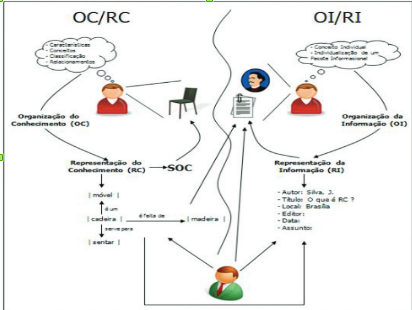
\includegraphics[scale=1.0]{figuras/figura-1}}
	}{
	\Fonte{\citeonline{smit2010temas}}
}
\end{figure}

\lipsum[1]

\begin{figure}[htbp]
	\centering
	\IBGEtab{
		\Caption{\label{figura-1}Ciclo da informação}		
    }{
		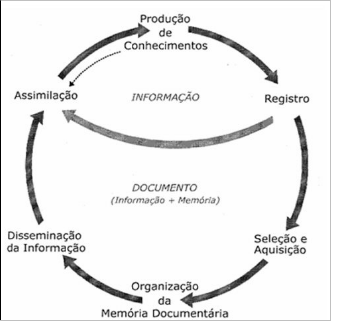
\includegraphics[scale=0.8]{figuras/figura-2}
	}{
	\Fonte{\citeonline{tristao2004sistema}}
}
\end{figure}



	%\chapter{Resultados}
\label{chap:resultados}

Implementamos o modelo produzido utilizando a linguagem de programação \textit{C++11} \cite{c++} em conjunto com o \textit{QT 5.2.1} \cite{qt} e o \textit{solver CPLEX 12.6.1} da \textit{IBM} \cite{ibmcplex} afim de avaliar o desempenho do modelo para instâncias de diferentes tamanhos. Escolhemos a linguagem \textit{C++} para preparar as instâncias para o \textit{CPLEX} por conta do seu alto desempenho. Utilizamos as bibliotecas de acesso aos dados do \textit{QT}, por apresentarem facilidade de uso. O \textit{CPLEX} foi utilizado por se tratar de um \textit{solver} robusto, que realiza de forma automática a conversão de restrições não lineares para restrições lineares e dá suporte a execução paralela (\textit{threads}), ambos recursos utilizados nos experimentos deste trabalho.

Todos os experimentos foram realizados em um computador com processador \textit{Intel(R) Xeon(R) CPU E31240 @ 3.30GHz}, 8 GB de memória RAM e com 8 GB na partição de \textit{swap}, executando o sistema operacional Ubuntu 14.04.5 LTS.

Os testes foram realizados sobre as ofertas de disciplinas da UFC-Quixadá do semestre 2016.2. Os dados contam com 108 ofertas de disciplinas divididas em 6 cursos. São ao todo 58 professores, e a preferência de um professor por uma disciplina foi dada pelo número de vezes que esse professor ministrou essa disciplina no campus. O número de alunos nos choques de horários das disciplinas é definido de forma aleatória, já que não foi possível conseguir essas informações para os testes. Primeiramente é atribuído a cada disciplina um valor entre 10 e 50 (incluindo os extremos) referente ao número de alunos que podem cursar cada disciplina. Depois, para cada par $(a, b)$ de disciplinas, sorteamos um valor entre 0 e o mínimo do número de alunos de $a$ e $b$ para definir a interseção de alunos entre as duas disciplinas. O valor definido para a interseção passa a ser então o número de alunos que podem cursar as duas disciplinas.

A partir do conjunto de dados obtido, utilizando a linguagem de programação \textit{Python 2.7} \cite{python} para automatizar o processamento dos dados, e o banco de dados \textit{SQLite 3.11} \cite{sqlite} para armazená-los, ambos escolhidos pela facilidade de uso. Preparamos aleatoriamente instâncias com diferentes proporções dos dados reais, ou seja, instâncias com 10\%, 20\%, ..., 90\% e 100\% dos professores e disciplinas escolhidos de forma aleatória (exemplo: 10\% dos professores e 10\% das disciplinas). Aplicamos essas instâncias para valores de $\alpha \in{\{0, 0.5, 1\}}$, e definimos um \textit{timeout} de 10 horas.

É importante lembrar que as alocações produzidas com $\alpha = 1$ não levam em consideração a preferência dos professores e são possivelmente alocações indesejáveis e não aplicáveis à UFC-Quixadá. Os testes realizados para esse valor têm intuito apenas de avaliar o desempenho do modelo quando são desconsideradas as preferências por disciplinas dos professores.

A Tabela \oldref{tabela-experimentos} apresenta o resultado dos experimentos para todas as instâncias. A primeira coluna se refere ao nome das instâncias, a segunda coluna ao valor $\alpha$ aplicado sobre as instâncias, a terceira ao tempo total de execução em segundos (\textit{real time + sync time + wait time + root node processing}, fornecidos pelo \textit{CPLEX}), e a quarta coluna apresenta o resultado obtido para cada teste.

\begin{table}[h!]
	\IBGEtab{
	\Caption{\label{tabela-experimentos} Tabela de Experimentos.}
	} &   0 &     1.46 & Ótimo \\
			                      & 0.5 &     0.30 & Ótimo \\
			                      &   1 &     0.25 & Ótimo \\
			\midrule
			\multirow{3}{*}{20\%} &   0 &     3.61 & Ótimo \\
			                      & 0.5 &  1943.68 & Ótimo \\
			                      &   1 &  1353.89 & Ótimo \\
			\midrule
			\multirow{3}{*}{30\%} &   0 &    13.51 & Ótimo \\
			                      & 0.5 &  1297.13 & Solução viável (Excedeu a memória) \\
			                      &   1 &  1701.42 & Solução viável (Excedeu a memória) \\
			\midrule
			\multirow{3}{*}{40\%} &   0 &    43.79 & Ótimo \\
			                      & 0.5 &  2255.91 & Solução viável (Excedeu a memória) \\
			                      &   1 &  2043.66 & Solução viável (Excedeu a memória) \\
			\midrule
			\multirow{3}{*}{50\%} &   0 &   195.00 & Ótimo \\
			                      & 0.5 &  3405.17 & Solução viável (Excedeu a memória)\\
			                      &   1 &  8915.71 & Solução viável (Excedeu a memória)\\
			\midrule
			\multirow{3}{*}{60\%} &   0 &   170.55 & Ótimo \\
			                      & 0.5 &  8008.68 & Solução viável (Excedeu a memória)\\
			                      &   1 & 20669.59 & Solução viável (Excedeu a memória)\\
			\midrule
			\multirow{3}{*}{70\%} &   0 &   375.21 & Ótimo \\
			                      & 0.5 &  9585.77 & Solução viável (Excedeu a memória)\\
			                      &   1 &  6608.70 & Nenhuma solução (Excedeu a memória) \\
			\midrule
			\multirow{3}{*}{80\%} &   0 &  3386.09 & Ótimo \\
			                      & 0.5 & 27010.67 & Solução viável (Excedeu a memória)\\
			                      &   1 &  9018.20 & Nenhuma solução (Excedeu a memória)\\
			\midrule
			\multirow{3}{*}{90\%} &   0 &  7369.57 & Nenhuma solução (Excedeu a memória)\\
			                      & 0.5 & 10763.45 & Nenhuma solução (Excedeu a memória)\\
			                      &   1 & 10153.70 & Nenhuma solução (Excedeu a memória)\\
			\midrule
			\multirow{3}{*}{100\%}&   0 &  4611.18 & Nenhuma solução (Excedeu a memória)\\
			                      & 0.5 & 36001.29 & Solução viável (Timeout) \\
			                      &   1 & 21974.03 & Nenhuma solução (Excedeu a memória)\\
			\bottomrule
		\end{tabular}%
	}{\Fonte{Produzido pelo autor}
	}
\end{table}

\newpage

Na Tabela \oldref{tabela-experimentos} podemos perceber que quando $\alpha = 0$, a implementação obteve soluções ótimas para as instâncias de tamanho até 80\% da oferta total do semestre 2016.2, mas para instâncias de maior tamanho, nenhuma solução foi encontrada. Para $\alpha = 0.5$, nenhuma solução ótima foi encontrada para as instâncias com mais de 20\% dos dados, mas obtivemos pelo menos uma solução viável para todas as instâncias com exceção da de 90\%. Para $\alpha = 1$, nenhuma solução ótima foi encontrada para as instâncias com mais de 20\%, e nas instâncias com mais de 60\% dos dados, não foi encontrada nenhuma solução viável.

Quanto às alocações geradas, nas instâncias menores ocorrem muitos casos em que professores são associados à disciplinas que estão fora da sua área de estudo, como por exemplo, um professor de otimização associado à disciplina de fotografia. Isso é esperado, pois sendo os professores e disciplinas escolhidos de forma aleatória para compor a instância, não temos a garantia de haver uma proporção adequada entre os professores de uma área de estudo e as disciplinas dessa mesma área. É importante lembrar, que essas instâncias tem o intuito apenas de avaliar o desempenho do modelo. Na solução viável encontrada para a instância com 100\% dos dados, a alocação de professores em disciplinas foi quase em sua totalidade semelhante às alocações que são aplicadas atualmente no campus. Apesar disso houveram algumas alocações aparentemente indesejáveis entre professores e disciplinas (professores alocados à disciplinas às quais não estão haptos a lecionar). Considerando que a solução encontrada não é a solução ótima, e que o programa parou por exceder o tempo limite de execução, isso já era esperado para essa situação.

Como ilustração, a Figura \oldref{figura-2} apresenta a alocação gerada para as disciplinas do quarto semestre do curso de Ciência da Computação para a instância com 100\% dos dados e $\alpha = 0.5$.

\begin{figure}[htbp]
	\centering
	\IBGEtab{
		\Caption{\label{figura-2}Alocação das disciplinas do quarto semestre do curso de Ciência da Computação}		
    }{
		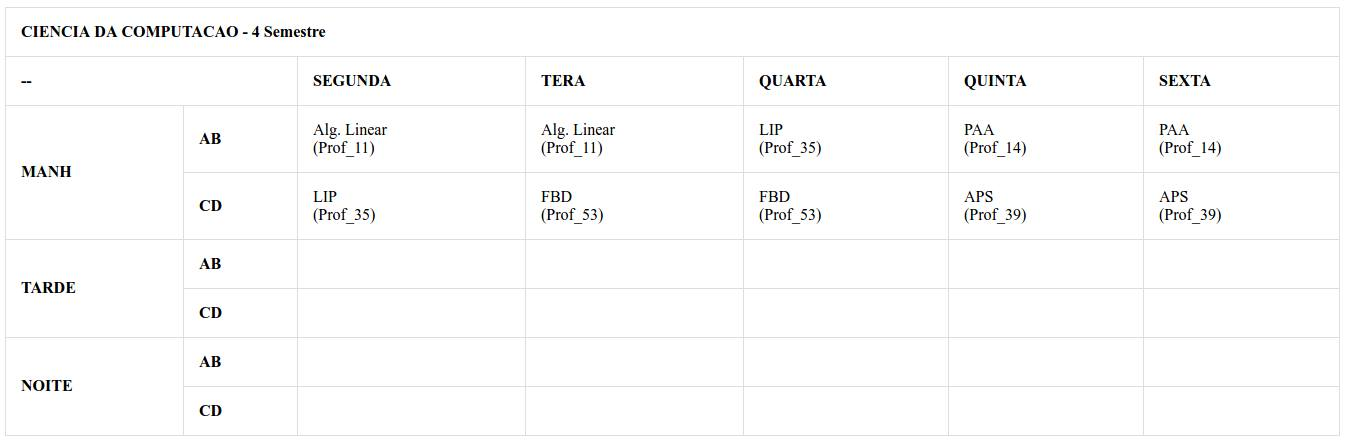
\includegraphics[scale=0.32]{figuras/alocacao}
	}{
	\Fonte{Elaborada pelo autor}
}
\end{figure}

	%\chapter{Discussão}
\label{chap:discussao}

A discussão consiste em destacar os principais resultados, bem como compará-los entre si.  Nesta Seção deve-se dar sentido ao que foi encontrado, relacionando com os objetivos do estudo, e considerando o ponto de vista escolhido para análise. 

O ponto de vista da análise deve estar em conformidade com o conteúdo da Seção de Fundamentação Teórica. Repetindo: a discussão deve estar embasada nos conceitos da fundamentação teórica, ou não terá sentido ter apresentado a fundamentação teórica no mesmo texto. Mais uma vez: é preciso verificar se os critérios de análise considerados estão explicitados na seção de revisão bibliográfica/fundamentação teórica.

Em algumas monografias, poderá ser conveniente unir a Resultados e Discussão em uma única Seção. A melhor escolha será aquela que permitir a melhor apresentação do trabalho realizado e suas contribuições. Mesmo nas situações em que a separação é mais conveniente, sugere-se que comecem a ser escritas separadamente para evitar que o conteúdo excessivo de um item não iniba o detalhamento da escrita do outro item.
	%\chapter{Considerações Finais}
\label{chap:consideracoes}

Parte final do texto na qual se apresentam as conclusões apoiadas no desenvolvimento do assunto. É a recapitulação sintética dos resultados obtidos. Pode apresentar recomendações e sugestões para pesquisas futuras.

Os objetivos gerais guiam todo o trabalho de redação das considerações finais. Sendo assim, pode-se começar relendo os objetivos e analisando se eles foram, ou não, comprovadamente atingidos ao longo do trabalho. 

Aqui apresentam-se os pontos positivos e negativos da jornada, sempre visando responder aos objetivos traçados na introdução da monografia.

Isaac Newton certa vez afirmou: “se vim mais longe foi por estar no ombro de gigantes”. Deve-se reconhecer, para este trabalho, a contribuição dos que o antecederam. Mostra-se de que forma autores pesquisados e trabalhos anteriores contribuíram para o desenvolvimento do seu trabalho.

É raro se encontrar citações nas considerações finais. Uma possibilidade é quando se deseja comparar os resultados obtidos com os resultados de outras pesquisas.  Por exemplo, em trabalhos de otimização de alguma coisa, e se chegou a resultados diferentes de que outro pesquisador, este outro pesquisador pode ser citado e ter seus resultados comparados com o que foi alcançado.

Responda à questão: qual a contribuição do seu trabalho? Para tanto, volte à introdução, veja a contribuição prometida para a pesquisa, e comente a contribuição agora com base nos resultados do trabalho.

Opine! Aproveite! Essa é uma rara chance em que você tem liberdade para expressar sua opinião sem precisar buscar fundamentação na bibliografia ou nos dados coletados.
Relacione os aspectos que ficaram de fora do escopo do seu trabalho, apresentando-os como sugestões de trabalhos futuros. Desta forma, outros pesquisadores poderão dar continuidade ao que você construiu

	%Elementos pós-textuais
	\begingroup
    \raggedright
	\bibliography{elementos-pos-textuais/referencias}
    \endgroup

	%\imprimirglossario %opcional
	\imprimirapendices
		% Adicione aqui os apendices do seu trabalho
		%% USE CAPSLOCK 
\apendice{LOREM IPSUM}

O que temos em nosso corpo: apêndice ou anexo? Apêndice contém o que foi desenvolvido pelo autor. Anexo contém o que foi criado por outros autores.

\label{ap:lorem-ipsum}

\lipsum[1]
		\apendice{MODELO DE CAPA}
\label{ap:modelo-de-capa}

\lipsum[1]

	\imprimiranexos
		% Adicione aqui os anexos do seu trabalho
		%% USE CAPSLOCK 
\anexo{EXEMPLO DE ANEXO}
\label{an:exemplo-de-anexo}

\lipsum[13]
		%% USE CAPSLOCK 
\anexo{DINÂMICA DAS CLASSES SOCIAIS}
\label{an:dinamica-das-classes-sociais}

\lipsum[14]
\index{AAA}
	%\imprimirindice %opcional

\end{document}
